\section{zmq-broker}

\begin{figure}
\centering
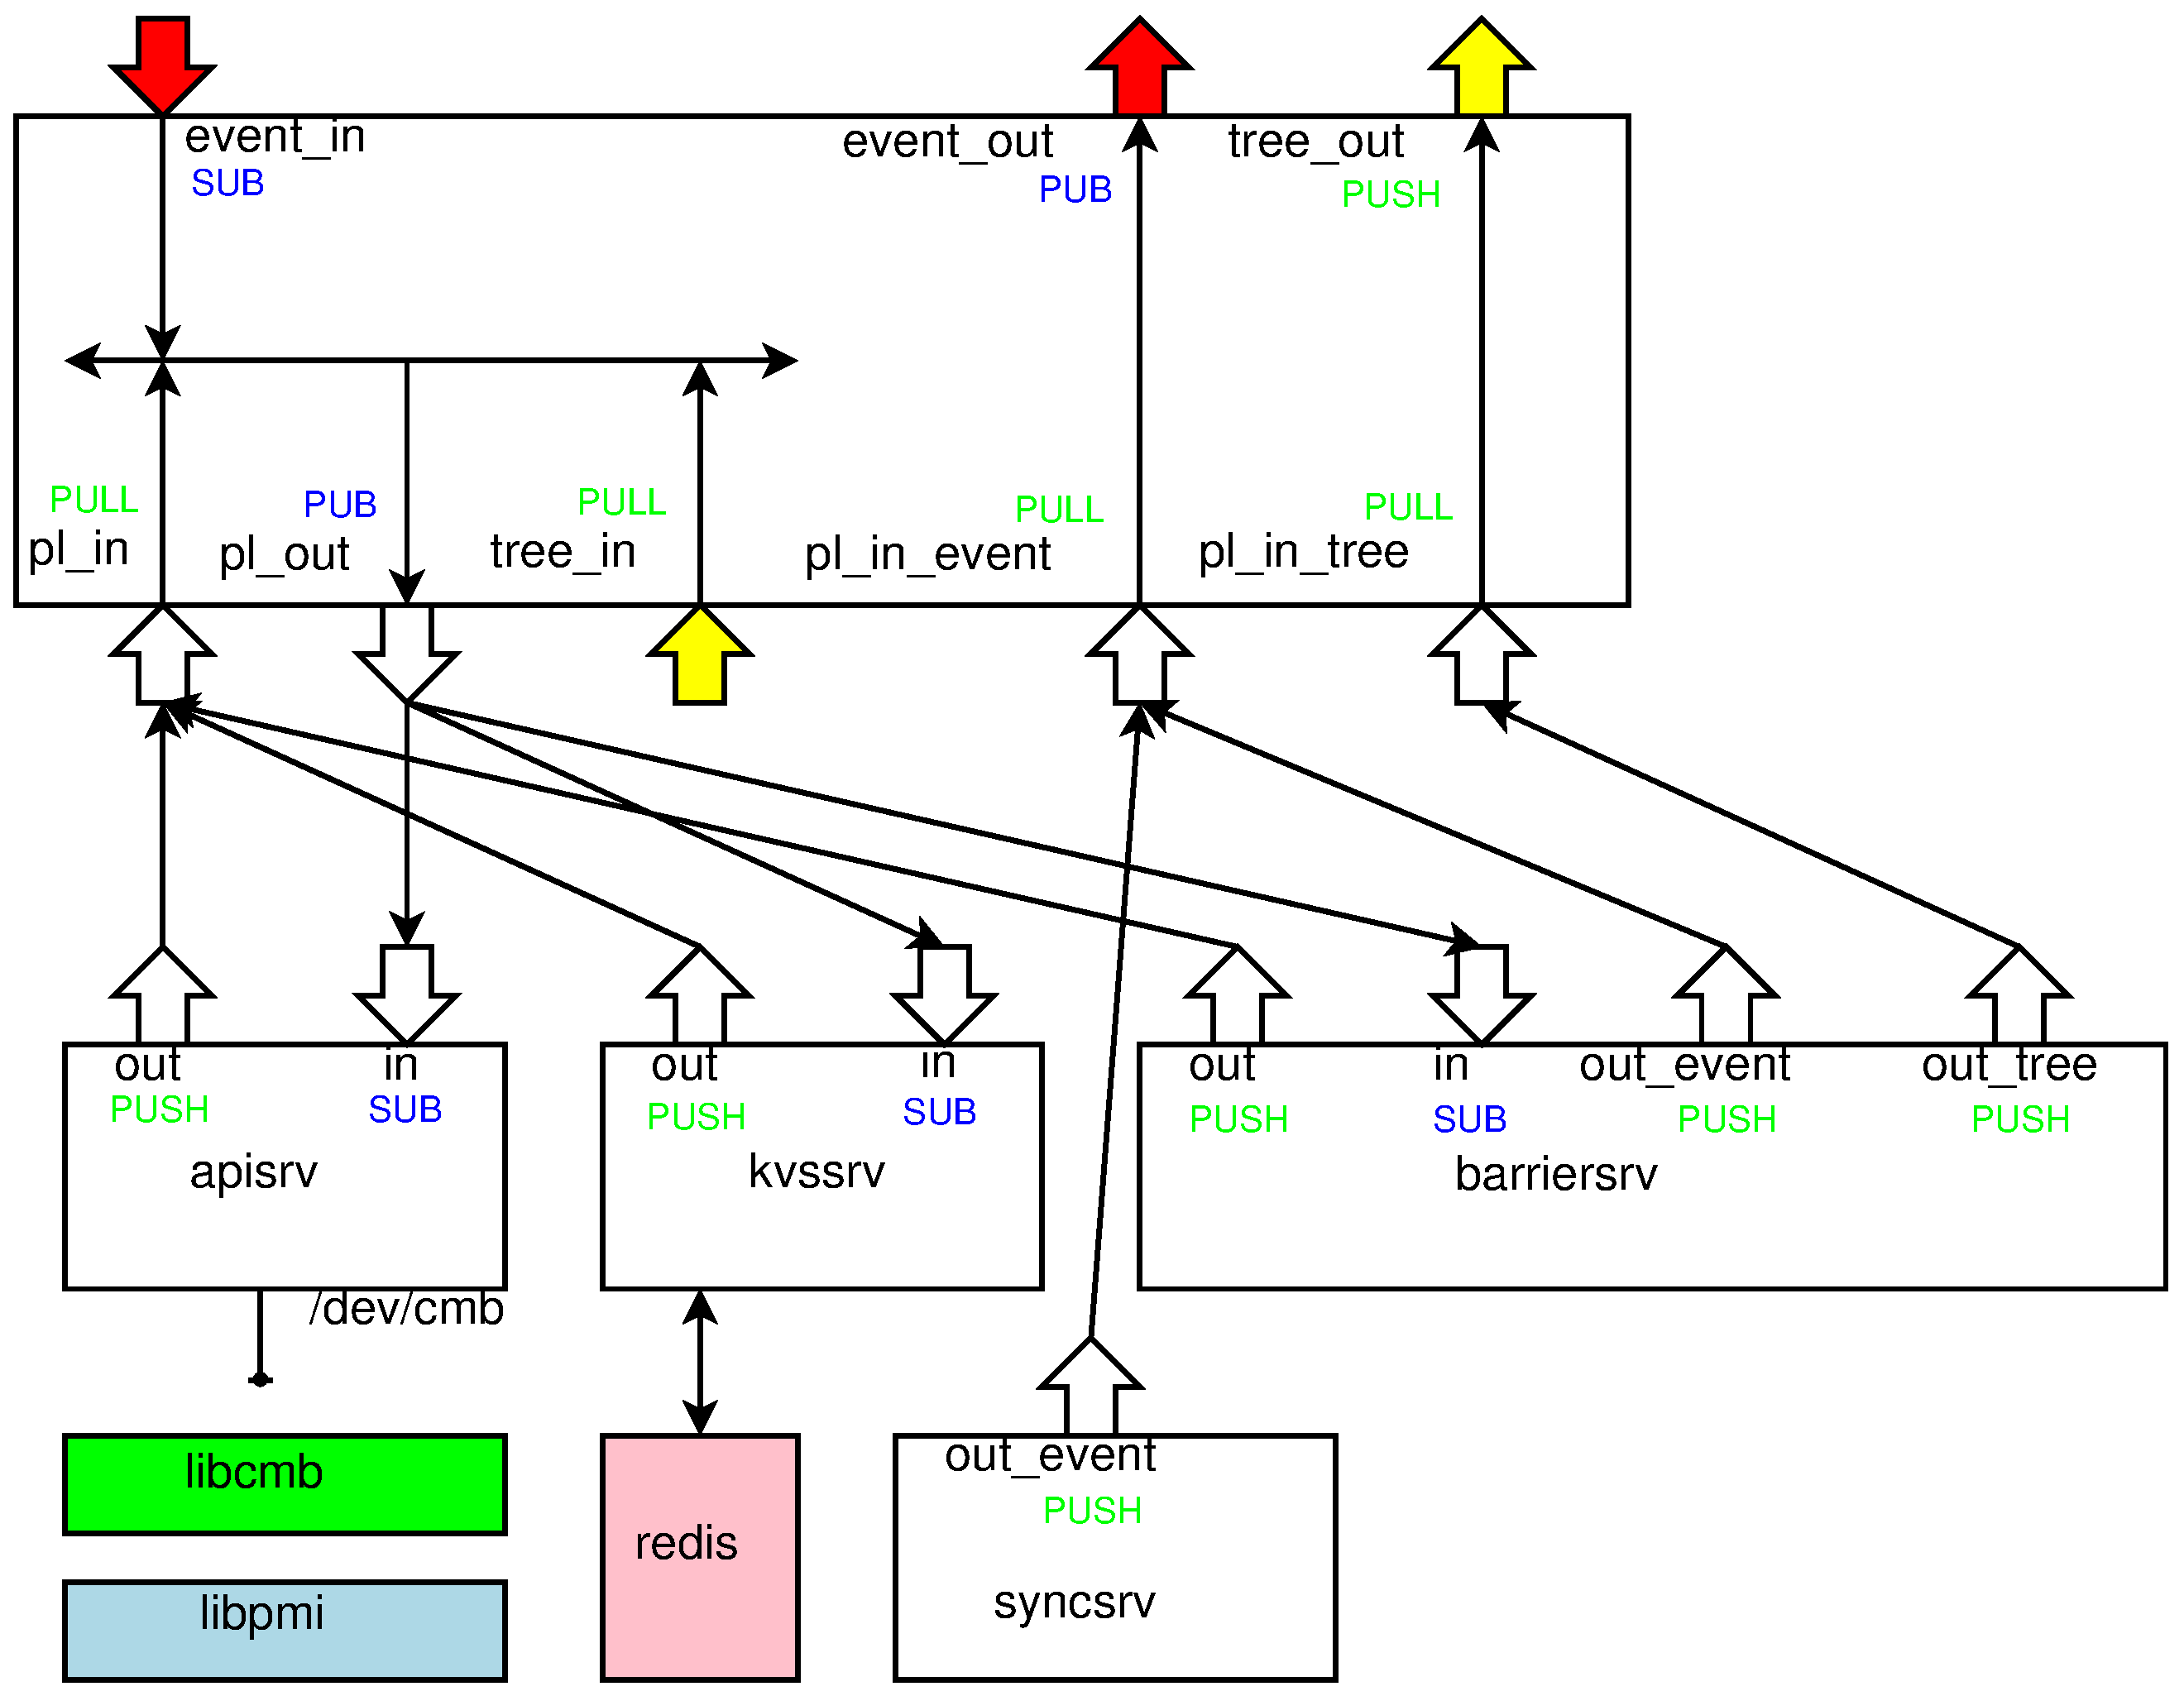
\includegraphics[scale=0.30]{zmq-broker.eps}
\caption{Broker internal architecture.  The cmbd simply routes messages
between \zMQ\ sockets, while plugins (syncsrv, apisrv, kvssrv, barriersrv)
perform specialized services.
Plugins are implemented as threads spawned by the cmbd, and communicate
with the cmbd using {\em inproc} (shared memory) \zMQ\ sockets.
The {\em libcmb} library, which provides the system's public interfaces,
communicates with the apisrv plugin via a UNIX domain socket.}
\label{fig:cmbint}
\end{figure}

\begin{figure}
\centering
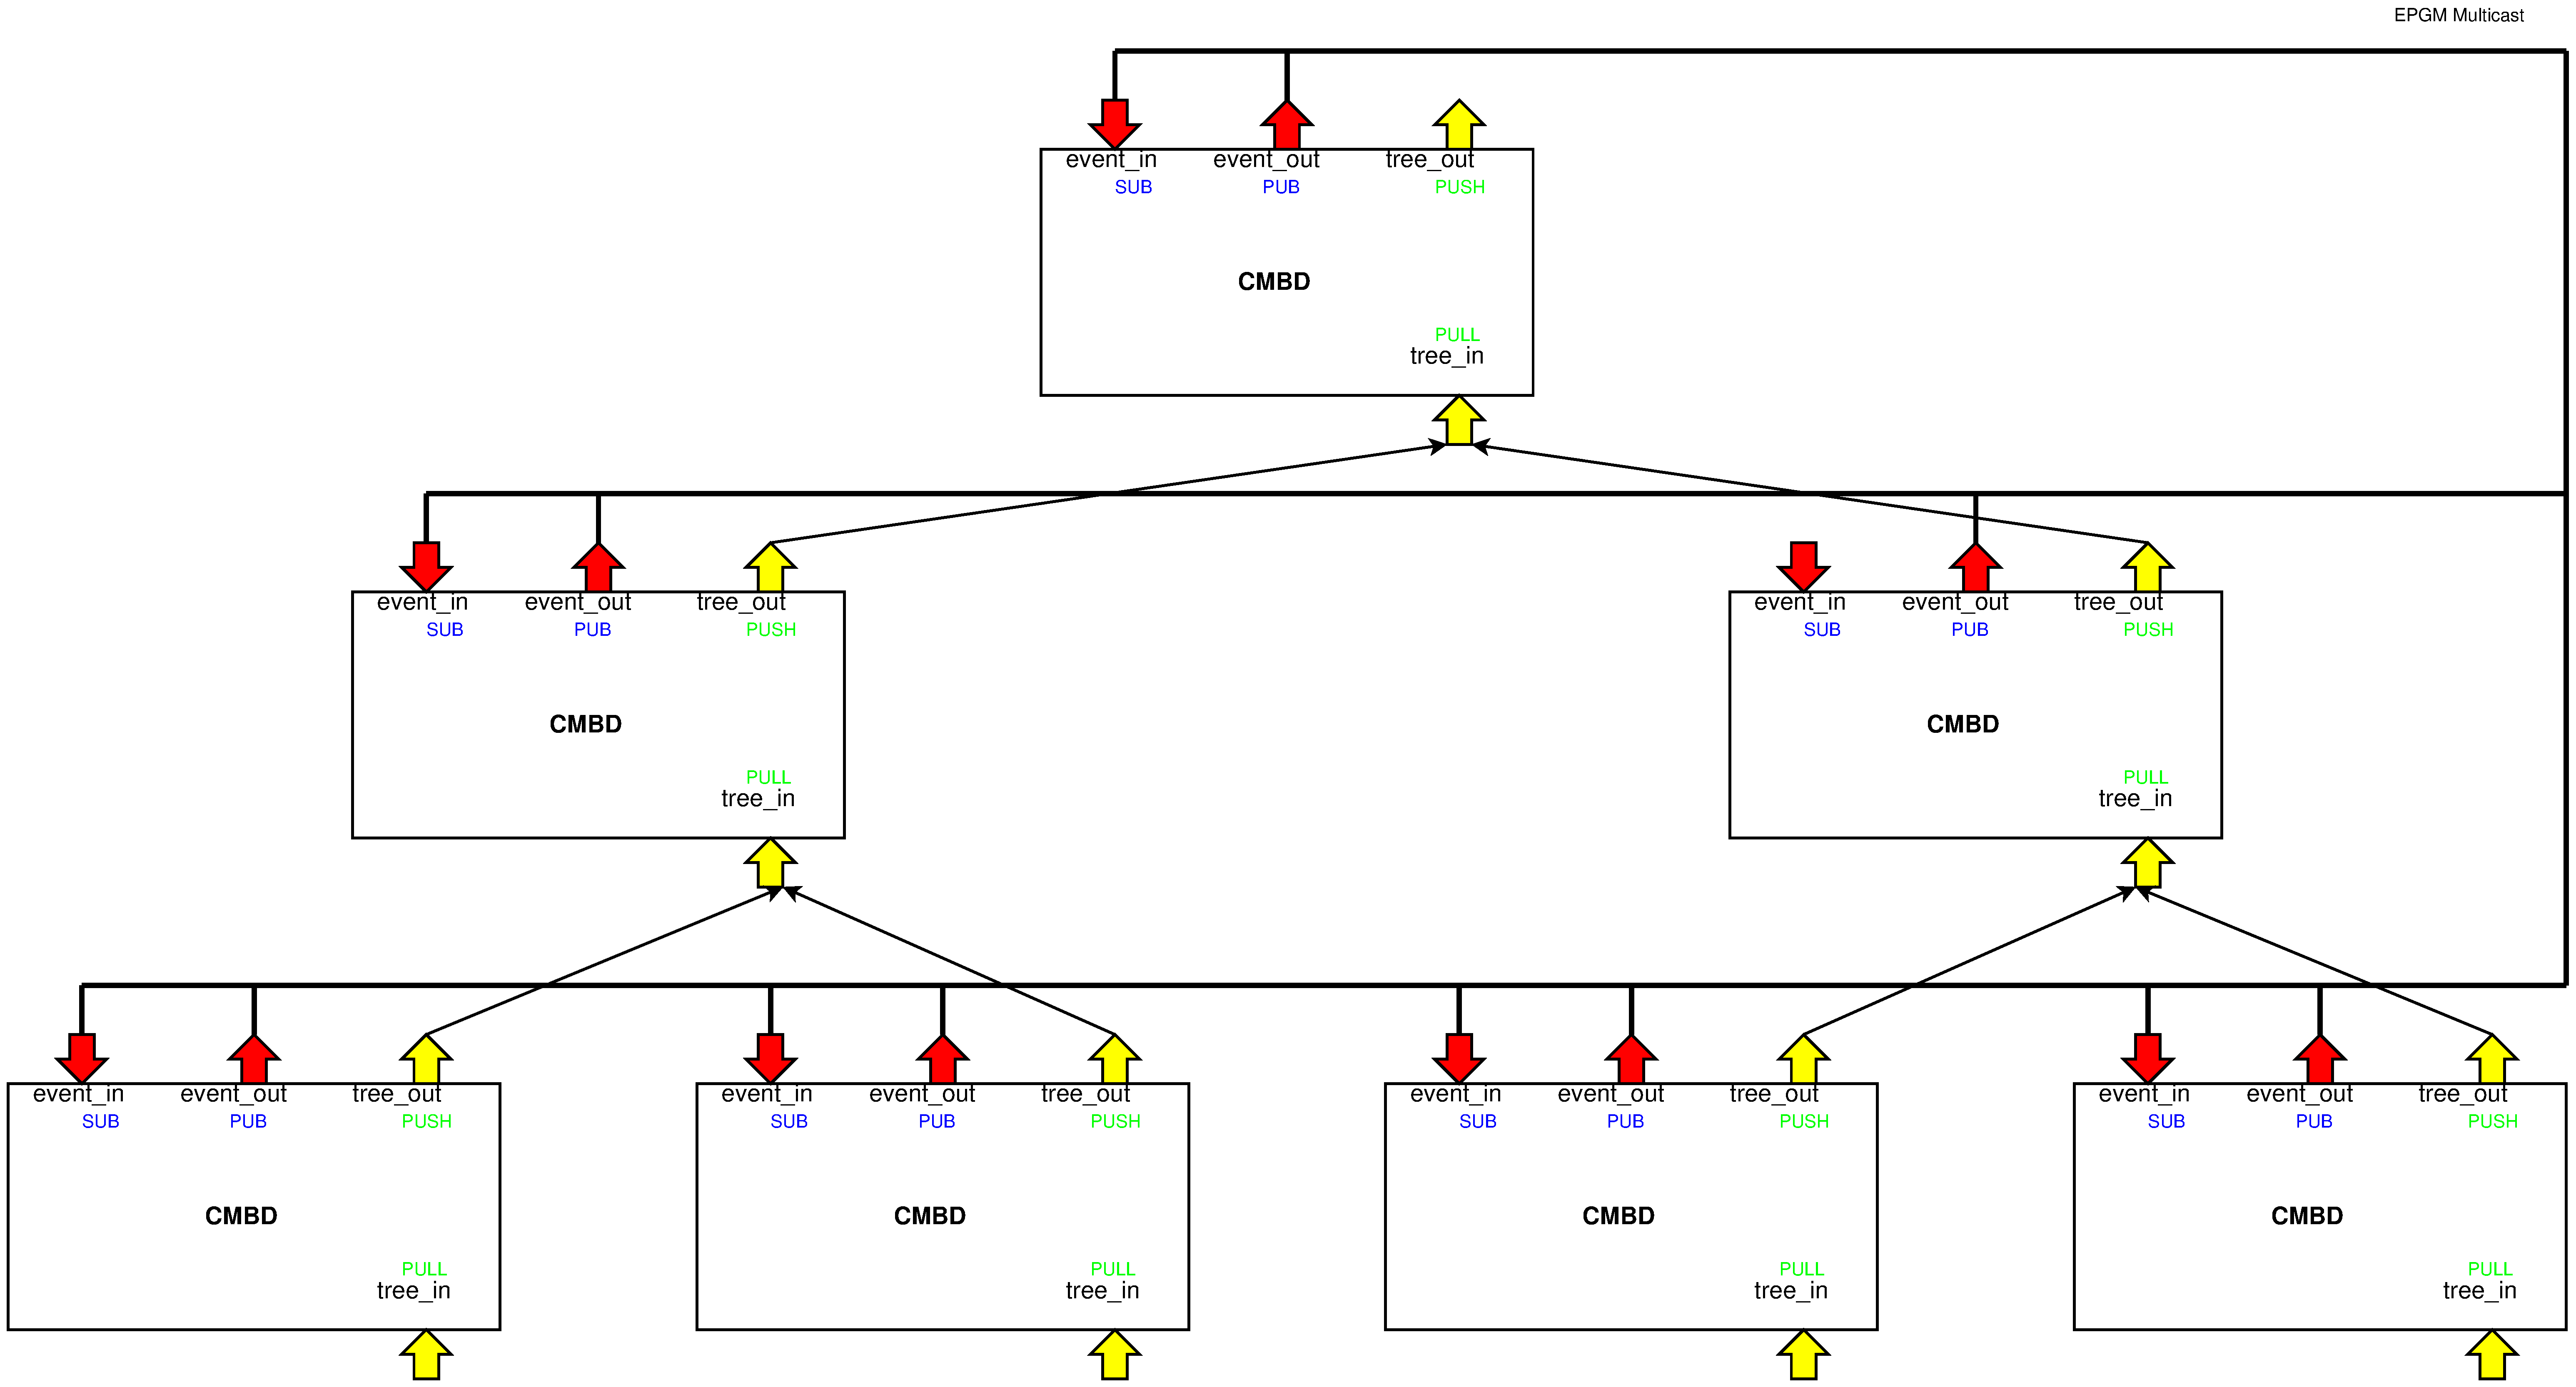
\includegraphics[scale=0.15]{zmq-broker-tree.eps}
\caption{Broker external architecture.}
\label{fig:cmbext}
\end{figure}

\begin{table}
\centering
\begin{tabular}{|l|l|l|l|}\hline
\textbf{Plugin-sock} & \textbf{CMB-sock} & \textbf{CMB-sock}
					 & \textbf{External} \\
\hline
out (PUSH)		& pl\_in (PULL)	& {\em BUS} & \\
out\_event (PUSH)  & pl\_in\_event (PULL) & event\_out (PUB) & $\rightarrow$ \\
out\_tree (PUSH) & pl\_in\_tree	(PULL) & tree\_out (PUSH) & $\rightarrow$ \\
in (SUB)	& pl\_out (PUB)	& {\em BUS}     & \\
\hline
		& {\em BUS}	& event\_in (SUB) & $\leftarrow$ \\
		& {\em BUS}	& tree\_in (PULL) & $\leftarrow$ \\
\hline
\end{tabular}
\caption{The cmbd internal routing table.}
\label{fig:cmbrouting}
\end{table}

\begin{table}
\centering
\begin{tabular}{|p{0.7cm}p{5cm}|p{9cm}|}\hline
\multicolumn{2}{|l|}{\textbf{Function}}
  & \textbf{Description} \\
\hline
{\tt cmb\_t} & {\tt cmb\_init (void)}
  & Create a {\em cmb\_t} context for communicating with the broker.\\
{\tt void} & {\tt cmb\_fini (cmb\_t c)}
  & Destroy a {\em cmb\_t} context.\\
\hline
{\tt int} & {\tt cmb\_ping (cmb\_t c, int seq, int padding)}
  & Send a ping message to the broker's internal bus and wait for it
    to be echoed back.  {\em padding} adds a json string of the specified
    length to the message.
    On success, returns $0$; on failure, returns $-1$ with errno set.\\
\hline
{\tt int} & {\tt cmb\_snoop (cmb\_t c, char {*sub})}
  & Print all messages on the broker's internal bus whose tags match the
    subscription string {\em sub}.  The empty string matches all messages.
    Returns $-1$ is returned with errno set.
    On success, does not return; on failure, returns $-1$ with errno set.\\
\hline
{\tt int}
  & {\tt cmb\_barrier (cmb\_t c, char {*name}, int nprocs,
                       int procs\_per\_node)}
  & Execute barrier {\em name}.  The call blocks until {\em nprocs}
    processes have entered the barrier.  If $procs\_per\_node < nprocs$
    then the tree network is used to resolve the barrier.
    On success, returns $0$; on failure, returns $-1$ with errno set.\\
\hline
{\tt int}
  & {\tt cmb\_sync (cmb\_t c)}
  & Block until {\em event.sched.trigger} is received.  This event is
    a job-wide, periodic multicast signal used to synchronize system noise.
    By default it is sent out every $10s$.
    On success, returns $0$; on failure, returns $-1$ with errno set.\\
\hline
{\tt int}
  & {\tt cmb\_kvs\_put (cmb\_t c, char {*key}, char {*val})}
  & Set {\em key} to {\em val} in the job-wide key-value store.
    If the key already has a value, it is overwritten.
    On success, returns $0$; on failure, returns $-1$ with errno set.\\
{\tt {char*}}
  & {\tt cmb\_kvs\_get (cmb\_t c, char {*key})}
  & Retrieve the value of {\em key} from the job-wide key-value store.
    On success, returns a copy of value which the caller must free;
    on failure, returns NULL with errno set.\\
{\tt int}
  & {\tt cmb\_kvs\_commit (cmb\_t c)}
  & Block until the job-wide key-value store has completed all transactions
    originating on the local node.
    On success, returns $0$; on failure, returns $-1$ with errno set.\\
\hline
\end{tabular}
\caption{Public interfaces exported by the broker.  Users would
{\tt \#include "cmb.h"} and link {\tt -lcmb}.}
\label{fig:cmbapi}
\end{table}


